% Nightly quota versus window budget. Illustrative sky pattern, not data.
% Generated by experiments/diagrams/build_diagrams.py -- edit the table there.
\documentclass[border=4pt]{standalone}
\usepackage{tikz}
\definecolor{plan}{HTML}{E69F00}
\definecolor{orbit}{HTML}{0072B2}
\definecolor{src}{HTML}{666666}
\colorlet{clear}{orbit!24}
\colorlet{partly}{src!30}
\colorlet{overcast}{src!65}
\begin{document}
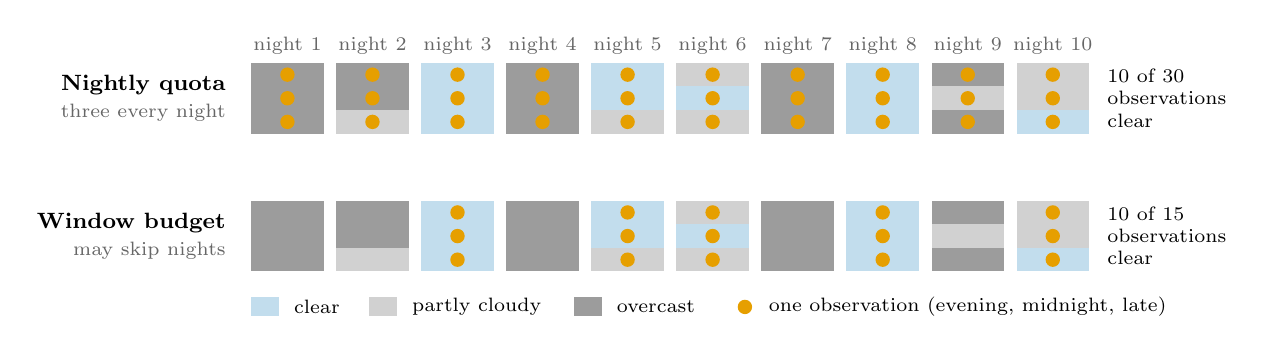
\begin{tikzpicture}[font=\footnotesize]
\node[anchor=east, align=right] at (-0.2,-0.45) {\textbf{Nightly quota}\\{\scriptsize\color{src}three every night}};
\fill[overcast] (0.00,-0.30) rectangle (0.92,0.00);
\fill[plan] (0.46,-0.15) circle (2.6pt);
\fill[overcast] (0.00,-0.60) rectangle (0.92,-0.30);
\fill[plan] (0.46,-0.45) circle (2.6pt);
\fill[overcast] (0.00,-0.90) rectangle (0.92,-0.60);
\fill[plan] (0.46,-0.75) circle (2.6pt);
\fill[overcast] (1.08,-0.30) rectangle (2.00,0.00);
\fill[plan] (1.54,-0.15) circle (2.6pt);
\fill[overcast] (1.08,-0.60) rectangle (2.00,-0.30);
\fill[plan] (1.54,-0.45) circle (2.6pt);
\fill[partly] (1.08,-0.90) rectangle (2.00,-0.60);
\fill[plan] (1.54,-0.75) circle (2.6pt);
\fill[clear] (2.16,-0.30) rectangle (3.08,0.00);
\fill[plan] (2.62,-0.15) circle (2.6pt);
\fill[clear] (2.16,-0.60) rectangle (3.08,-0.30);
\fill[plan] (2.62,-0.45) circle (2.6pt);
\fill[clear] (2.16,-0.90) rectangle (3.08,-0.60);
\fill[plan] (2.62,-0.75) circle (2.6pt);
\fill[overcast] (3.24,-0.30) rectangle (4.16,0.00);
\fill[plan] (3.70,-0.15) circle (2.6pt);
\fill[overcast] (3.24,-0.60) rectangle (4.16,-0.30);
\fill[plan] (3.70,-0.45) circle (2.6pt);
\fill[overcast] (3.24,-0.90) rectangle (4.16,-0.60);
\fill[plan] (3.70,-0.75) circle (2.6pt);
\fill[clear] (4.32,-0.30) rectangle (5.24,0.00);
\fill[plan] (4.78,-0.15) circle (2.6pt);
\fill[clear] (4.32,-0.60) rectangle (5.24,-0.30);
\fill[plan] (4.78,-0.45) circle (2.6pt);
\fill[partly] (4.32,-0.90) rectangle (5.24,-0.60);
\fill[plan] (4.78,-0.75) circle (2.6pt);
\fill[partly] (5.40,-0.30) rectangle (6.32,0.00);
\fill[plan] (5.86,-0.15) circle (2.6pt);
\fill[clear] (5.40,-0.60) rectangle (6.32,-0.30);
\fill[plan] (5.86,-0.45) circle (2.6pt);
\fill[partly] (5.40,-0.90) rectangle (6.32,-0.60);
\fill[plan] (5.86,-0.75) circle (2.6pt);
\fill[overcast] (6.48,-0.30) rectangle (7.40,0.00);
\fill[plan] (6.94,-0.15) circle (2.6pt);
\fill[overcast] (6.48,-0.60) rectangle (7.40,-0.30);
\fill[plan] (6.94,-0.45) circle (2.6pt);
\fill[overcast] (6.48,-0.90) rectangle (7.40,-0.60);
\fill[plan] (6.94,-0.75) circle (2.6pt);
\fill[clear] (7.56,-0.30) rectangle (8.48,0.00);
\fill[plan] (8.02,-0.15) circle (2.6pt);
\fill[clear] (7.56,-0.60) rectangle (8.48,-0.30);
\fill[plan] (8.02,-0.45) circle (2.6pt);
\fill[clear] (7.56,-0.90) rectangle (8.48,-0.60);
\fill[plan] (8.02,-0.75) circle (2.6pt);
\fill[overcast] (8.64,-0.30) rectangle (9.56,0.00);
\fill[plan] (9.10,-0.15) circle (2.6pt);
\fill[partly] (8.64,-0.60) rectangle (9.56,-0.30);
\fill[plan] (9.10,-0.45) circle (2.6pt);
\fill[overcast] (8.64,-0.90) rectangle (9.56,-0.60);
\fill[plan] (9.10,-0.75) circle (2.6pt);
\fill[partly] (9.72,-0.30) rectangle (10.64,0.00);
\fill[plan] (10.18,-0.15) circle (2.6pt);
\fill[partly] (9.72,-0.60) rectangle (10.64,-0.30);
\fill[plan] (10.18,-0.45) circle (2.6pt);
\fill[clear] (9.72,-0.90) rectangle (10.64,-0.60);
\fill[plan] (10.18,-0.75) circle (2.6pt);
\node[anchor=west, align=left, font=\scriptsize] at (10.75,-0.45) {10 of 30\\observations\\clear};
\node[anchor=east, align=right] at (-0.2,-2.20) {\textbf{Window budget}\\{\scriptsize\color{src}may skip nights}};
\fill[overcast] (0.00,-2.05) rectangle (0.92,-1.75);
\fill[overcast] (0.00,-2.35) rectangle (0.92,-2.05);
\fill[overcast] (0.00,-2.65) rectangle (0.92,-2.35);
\fill[overcast] (1.08,-2.05) rectangle (2.00,-1.75);
\fill[overcast] (1.08,-2.35) rectangle (2.00,-2.05);
\fill[partly] (1.08,-2.65) rectangle (2.00,-2.35);
\fill[clear] (2.16,-2.05) rectangle (3.08,-1.75);
\fill[plan] (2.62,-1.90) circle (2.6pt);
\fill[clear] (2.16,-2.35) rectangle (3.08,-2.05);
\fill[plan] (2.62,-2.20) circle (2.6pt);
\fill[clear] (2.16,-2.65) rectangle (3.08,-2.35);
\fill[plan] (2.62,-2.50) circle (2.6pt);
\fill[overcast] (3.24,-2.05) rectangle (4.16,-1.75);
\fill[overcast] (3.24,-2.35) rectangle (4.16,-2.05);
\fill[overcast] (3.24,-2.65) rectangle (4.16,-2.35);
\fill[clear] (4.32,-2.05) rectangle (5.24,-1.75);
\fill[plan] (4.78,-1.90) circle (2.6pt);
\fill[clear] (4.32,-2.35) rectangle (5.24,-2.05);
\fill[plan] (4.78,-2.20) circle (2.6pt);
\fill[partly] (4.32,-2.65) rectangle (5.24,-2.35);
\fill[plan] (4.78,-2.50) circle (2.6pt);
\fill[partly] (5.40,-2.05) rectangle (6.32,-1.75);
\fill[plan] (5.86,-1.90) circle (2.6pt);
\fill[clear] (5.40,-2.35) rectangle (6.32,-2.05);
\fill[plan] (5.86,-2.20) circle (2.6pt);
\fill[partly] (5.40,-2.65) rectangle (6.32,-2.35);
\fill[plan] (5.86,-2.50) circle (2.6pt);
\fill[overcast] (6.48,-2.05) rectangle (7.40,-1.75);
\fill[overcast] (6.48,-2.35) rectangle (7.40,-2.05);
\fill[overcast] (6.48,-2.65) rectangle (7.40,-2.35);
\fill[clear] (7.56,-2.05) rectangle (8.48,-1.75);
\fill[plan] (8.02,-1.90) circle (2.6pt);
\fill[clear] (7.56,-2.35) rectangle (8.48,-2.05);
\fill[plan] (8.02,-2.20) circle (2.6pt);
\fill[clear] (7.56,-2.65) rectangle (8.48,-2.35);
\fill[plan] (8.02,-2.50) circle (2.6pt);
\fill[overcast] (8.64,-2.05) rectangle (9.56,-1.75);
\fill[partly] (8.64,-2.35) rectangle (9.56,-2.05);
\fill[overcast] (8.64,-2.65) rectangle (9.56,-2.35);
\fill[partly] (9.72,-2.05) rectangle (10.64,-1.75);
\fill[plan] (10.18,-1.90) circle (2.6pt);
\fill[partly] (9.72,-2.35) rectangle (10.64,-2.05);
\fill[plan] (10.18,-2.20) circle (2.6pt);
\fill[clear] (9.72,-2.65) rectangle (10.64,-2.35);
\fill[plan] (10.18,-2.50) circle (2.6pt);
\node[anchor=west, align=left, font=\scriptsize] at (10.75,-2.20) {10 of 15\\observations\\clear};
\node[font=\scriptsize, text=src] at (0.46,0.22) {night 1};
\node[font=\scriptsize, text=src] at (1.54,0.22) {night 2};
\node[font=\scriptsize, text=src] at (2.62,0.22) {night 3};
\node[font=\scriptsize, text=src] at (3.70,0.22) {night 4};
\node[font=\scriptsize, text=src] at (4.78,0.22) {night 5};
\node[font=\scriptsize, text=src] at (5.86,0.22) {night 6};
\node[font=\scriptsize, text=src] at (6.94,0.22) {night 7};
\node[font=\scriptsize, text=src] at (8.02,0.22) {night 8};
\node[font=\scriptsize, text=src] at (9.10,0.22) {night 9};
\node[font=\scriptsize, text=src] at (10.18,0.22) {night 10};
\fill[clear] (0.00,-3.22) rectangle (0.35,-2.98);
\node[anchor=west, font=\scriptsize] at (0.42,-3.10) {clear};
\fill[partly] (1.50,-3.22) rectangle (1.85,-2.98);
\node[anchor=west, font=\scriptsize] at (1.92,-3.10) {partly cloudy};
\fill[overcast] (4.10,-3.22) rectangle (4.45,-2.98);
\node[anchor=west, font=\scriptsize] at (4.52,-3.10) {overcast};
\fill[plan] (6.27,-3.10) circle (2.6pt);
\node[anchor=west, font=\scriptsize] at (6.45,-3.10) {one observation (evening, midnight, late)};
\end{tikzpicture}
\end{document}
